\documentclass[11pt]{amsart}
\usepackage[a4paper,textwidth=158mm,textheight=237mm,centering]{geometry}
\usepackage[T1]{fontenc}
\usepackage{lmodern,microtype,mathtools,amssymb,graphicx,flafter,booktabs}
\usepackage{tikz}
\usepackage[unicode,colorlinks=true,linkcolor=black,citecolor=black,urlcolor=blue]{hyperref}
\newtheorem{theorem}{Theorem}[section]
\newtheorem{lemma}[theorem]{Lemma}
\newtheorem{proposition}[theorem]{Proposition}
\newtheorem{corollary}[theorem]{Corollary}
\theoremstyle{definition}
\newtheorem{definition}[theorem]{Definition}
\theoremstyle{remark}
\newtheorem{remark}[theorem]{Remark}
\newcommand{\Hex}{\mathrm{Hex}}
\Urlmuskip=0mu plus 1mu
\def\UrlBreaks{\do\/\do-\do\_}
\newcommand{\W}{\mathcal W}
\title{Short forced wins in small Hex}
\author{Harvey Yorke}
\address{Valyu AI}
\ifdefined\journalversion\else
\author{Valyu DeepResearch}
\address{Valyu AI}
\fi
\ifdefined\journalversion
  \hypersetup{pdftitle={Short forced wins in small Hex},pdfauthor={Harvey Yorke}}
\else
  \hypersetup{pdftitle={Short forced wins in small Hex},pdfauthor={Harvey Yorke and Valyu DeepResearch}}
\fi
\date{25 October 2026}
\keywords{Hex, Maker-Breaker games, game solving, computer-assisted proof}
\newcommand{\paperAuthorBlock}[1]{%
  \begin{minipage}[t]{.44\textwidth}
    \centering\normalfont\normalsize #1\par\small Valyu AI\par
  \end{minipage}%
}
\makeatletter
\renewcommand{\@setauthors}{%
  \begingroup\trivlist\centering\normalfont\normalsize
  \@topsep30\p@\relax\advance\@topsep by -\baselineskip\item\relax
  \ifdefined\journalversion
    \paperAuthorBlock{Harvey Yorke}%
  \else
    \paperAuthorBlock{Harvey Yorke}\hspace{.06\textwidth}\paperAuthorBlock{Valyu DeepResearch}%
  \fi
  \endtrivlist\endgroup
}
\renewcommand{\@setaddresses}{}
\makeatother
\begin{document}
\raggedbottom
\begin{abstract}
Campbell (2004) asked for the shortest path $\lambda(n)$ with which the first player can force a win in $n\times n$ Hex, and for the fewest stones $\delta(n)$ with which the first player can force a win. He conjectured $\lambda(5)=\delta(5)=7$ and $\lambda(6)=\delta(6)=9$. A 2026 preprint announces a proof that $\lambda(5)=7$ and conjectures $\lambda(6)=\delta(6)=9$. We settle the small cases by exhaustive Maker-Breaker search with certificates that an independent checker replays. Opening in the centre of the $5\times5$ board, the first player can force a winning path of six cells, so $\lambda(5)=6$. This holds under Campbell's rules and also when play stops at the first connection. We also prove $\delta(5)=7$, $\delta(6)=10$ and $\lambda(6)\ge8$, and our search gives $\lambda(6)=8$ under Campbell's rules. Thus the two parameters already differ at $n=5$, the conjecture $\delta(6)=9$ fails, and by our search so does $\lambda(6)=9$. The value $\delta(6)=10$ agrees with an earlier non-exhaustive estimate from a self-play Hex program.
\end{abstract}
\maketitle

\section{The question}

Hex is played on an $n\times n$ rhombus of hexagonal cells. Blue moves first and tries to join the top and bottom rows with a chain of blue cells; Red tries to join the left and right columns. A finished board has exactly one winner~\cite{Gale1979}, and strategy stealing shows that the first player can force a win. Campbell~\cite{Campbell2004} asked how cheap such a win can be made, and introduced two measures.

\begin{definition}[Campbell]\label{def:games}
In $\Hex(n,l)$, Blue wins only by constructing a top-bottom path of at most $l$ cells. If Blue's stones join the two blue rows only by longer paths, play continues while Blue can still make a short path. In $\Hex_d(n)$, Blue must win ordinary Hex having placed at most $d$ stones. Put
\begin{align*}
\lambda(n)&=\min\{l:\text{Blue can force a win in }\Hex(n,l)\},\\
\delta(n)&=\min\{d:\text{Blue can force a win in }\Hex_d(n)\}.
\end{align*}
\end{definition}

Campbell's rule that play continues after a long connection is explicit: with a long Blue connection on the board, ``play would continue since the Hex(4) winning path is not with a path of length less than or equal to 5 and since blue still has a chance of winning with such a path''~\cite[\S2]{Campbell2004}. A winning set of $d$ stones contains a path of at most $d$ cells, so $\lambda(n)\le\delta(n)$, and Campbell notes that the depth of Hex is $2\delta(n)-1$. He proved $\lambda(n)>n$ for $n\ge4$ and $\delta(n)\ge n+\lfloor n/4\rfloor$, and, using strategies known since 1959~\cite{Gardner1959}, $\lambda(4)=\delta(4)=5$, $6\le\lambda(5)\le7$ and $6\le\delta(5)\le7$~\cite[Corollaries 12, 13, Theorems 14, 15]{Campbell2004}. Stromquist~\cite{Stromquist2007} proved $\lambda(n)\ge n+\lfloor (n-2)/4\rfloor$. Campbell conjectured~\cite[Conjectures 19, 20]{Campbell2004}
\[
\lambda(5)=7,\quad \lambda(6)=9,\qquad \delta(5)=7,\quad \delta(6)=9.
\]
Casco, Pacifico and Sanhueza~\cite{CPS2026} announce a proof by case analysis that $\lambda(5)=7$ (their Theorem~A), deduce $\delta(5)=7$, and list as ``the most immediate open problem'' the exact values of $\lambda(6)$ and $\delta(6)$, conjecturing $\lambda(6)=\delta(6)=9=2n-3$. They also ask whether $\lambda(n)=\delta(n)$ for all $n$.

Their definition of $\lambda$ is phrased through ``every resulting winning path'' of an ordinary Hex game, which ends at the first connection. We therefore also consider the \emph{strict} game $\Hex^{*}(n,l)$: ordinary Hex, in which Blue succeeds if Blue makes the first connection and that connection contains a top-bottom path of at most $l$ cells. A strict success is a success in $\Hex(n,l)$, so the strict value $\lambda^{*}(n)$ satisfies $\lambda(n)\le\lambda^{*}(n)\le\delta(n)$.

\begin{theorem}\label{thm:main}
\begin{enumerate}
\item $\lambda(5)=\lambda^{*}(5)=6$. Opening in the centre, Blue can ensure that its first connection contains a top-bottom path of at most six cells. Red can prevent every Blue path of at most five cells, whatever Blue's opening.
\item $\delta(5)=7$.
\item $\delta(6)=10$. Red can stop every Blue connection made with nine or fewer stones, whatever Blue's opening. Blue wins with at most ten stones by opening in either of the two central cells of the short diagonal.
\item $\lambda(6)\ge8$. Red can prevent every Blue path of at most seven cells, whatever Blue's opening.
\end{enumerate}
\end{theorem}

Each statement is proved by a finite certificate: a strategy for one player, given as a table of moves, that an independent program replays against every possible reply of the other player (Section~\ref{sec:cert}). Our search also gives the matching upper bound for $\lambda(6)$, which we have not certified in the same way.

\begin{proposition}[computation]\label{prop:lambda6}
Under Campbell's rules Blue forces a path of at most eight cells on the $6\times6$ board by opening at $(3,4)$, so $\lambda(6)=8$.
\end{proposition}

\begin{corollary}\label{cor:consequences}
Campbell's conjectured values fail for $\lambda(5)$ and $\delta(6)$, and, by Proposition~\ref{prop:lambda6}, for $\lambda(6)$. Theorem~A of~\cite{CPS2026} and its Lemma~5, which asserts that every strategy opening in the centre of the $5\times5$ board leaves Red a defence forcing a path of at least seven cells, are false under either reading of the rules. Since $\lambda(5)=6<7=\delta(5)$, the two parameters already differ at $n=5$, which answers the question of~\cite{CPS2026} whether $\lambda(n)=\delta(n)$ for all $n$. The proposed pattern $\lambda(n)=\delta(n)=2n-3$ fails for $\lambda$ at $n=5$ and for $\delta$ at $n=6$.
\end{corollary}

The conclusion $\delta(5)=7$ of~\cite{CPS2026} is correct, but their deduction from $\lambda(5)=7$ is not; part~(2) of Theorem~\ref{thm:main} gives a separate proof. For $\delta(6)$ there is earlier numerical evidence. KataHex, a self-play Hex program, estimated the optimal length of $6\times6$ Hex, with the first player hurrying and the second delaying, at $19$ moves~\cite{HZY2024,Irving2018}. By Campbell's relation this corresponds to $\delta(6)=10$. Its author states that this is ``NOT a exhaustive search'' and ``can't be called a proof''. Theorem~\ref{thm:main}(3) proves the value.

\section{The games as Maker-Breaker games}\label{sec:mb}

Label the cells $(r,c)$ with $1\le r,c\le n$. The neighbours of $(r,c)$ are $(r,c\pm1)$, $(r-1,c)$, $(r-1,c+1)$, $(r+1,c-1)$ and $(r+1,c)$; Blue's rows are $r=1$ and $r=n$, and the obtuse corners are $(1,n)$ and $(n,1)$. The only symmetry of the board that preserves Blue's rows is the half-turn $(r,c)\mapsto(n+1-r,n+1-c)$, so there are $\lceil n^2/2\rceil$ openings up to symmetry. Campbell~\cite{Campbell2004} and~\cite{CPS2026} label cells by row and column with Blue joining the left and right sides; the transposition $(r,c)\mapsto(c,r)$ converts their labels to ours, and the optimal openings reported below form sets invariant under it.

A \emph{top-bottom connection} is a set of cells containing a chain from row $1$ to row $n$. Let $\W_l$ be the family of inclusion-minimal top-bottom connections with at most $l$ cells. Each member is the cell set of a path, and $|\W_5|=48$, $|\W_6|=106$ and $|\W_7|=164$ on the $5\times5$ board; on the $6\times6$ board $|\W_7|=306$, $|\W_8|=560$, $|\W_9|=848$ and $|\W_{10}|=1301$.

\begin{lemma}\label{lem:mb}
\begin{enumerate}
\item Blue can force a win in $\Hex(n,l)$ if and only if Maker, moving first, wins the Maker-Breaker game on $\W_l$, in which Maker wins by claiming all cells of some member of $\W_l$.
\item Blue can force a win in $\Hex_d(n)$ if and only if Maker can claim a member of $\W_d$ before claiming more than $d$ cells.
\end{enumerate}
\end{lemma}

\begin{proof}
Blue's stones contain a top-bottom path of at most $l$ cells exactly when they contain a member of $\W_l$. If Red completes a left-right chain, every top-bottom path meets a red cell, because a left-right chain separates the top row from the bottom row; so every member of $\W_l$ is then dead, and stopping the game at that moment does not change whether Blue can still succeed. Hence the only effect of Red's own winning condition is already accounted for by Breaker's blocking. In $\Hex_d(n)$ a connection made with at most $d$ stones contains a minimal one with at most $d$ cells.
\end{proof}

In the strict game $\Hex^{*}(n,l)$ Blue additionally fails as soon as its stones form a top-bottom connection that contains no member of $\W_l$. Extra Blue stones can now hurt Blue, so the usual Maker monotonicity is unavailable; our strict computations use only the rules themselves (Section~\ref{sec:cert}).

\section{Search and certificates}\label{sec:cert}

\paragraph{Search.} A depth-first Maker-Breaker search with a transposition table decides each game. Positions are reduced as follows. Call a winning set \emph{live} if it contains no red cell and, in $\Hex_d(n)$, has at most as many empty cells as Blue has stones left. A cell on no live set is \emph{dead}; a move there is equivalent to passing, which never helps either player in a Maker-Breaker game~\cite{Beck2008}, so both players are restricted to cells on live sets. Breaker must answer a set with a single empty cell, and loses to two such cells. If Maker, moving twice, could create two completion cells by playing $v$, Breaker must play in $v$ or one of those cells. Finally, if every live set through $x$ also passes through $y$, Breaker's move at $y$ is at least as good as at $x$. These rules only remove moves that cannot change the outcome; in any case the proofs rest only on the certificates below. Separate implementations reproduce parts of the results: a plain search over top-bottom walks finds the centre win in $\Hex(5,6)$, a walk-based search with null-move pruning finds that Red holds $\Hex_9(6)$ after all $36$ openings, and a strict-game solver keyed on exact positions finds the centre win in $\Hex^{*}(5,6)$.

\paragraph{Keys.} Let $m$ be the number of stones Blue has left in $\Hex_d(n)$ ($m=\infty$ in $\Hex(n,l)$), and let $R$ be the union of the live sets. Since $R$ contains no red cell, the live sets are exactly the winning sets $W\subseteq R$ with $|W\setminus B|\le m$, where $B$ is the set of Blue cells; so the triple $(m,B\cap R,R)$ determines the live family. A set that is not live never becomes live, so a move outside $R$ changes no live set and acts as a pass (in $\Hex_d(n)$ it also uses one of Blue's stones). A pass never helps in a Maker-Breaker game: the player facing it can pretend that the opponent occupied some empty cell of $R$, follow the strategy, and repeat the pretence whenever the opponent later plays on a pretended cell; the real position is then always at least as good for that player as the pretended one. Hence if a player wins from one position, that player wins from every position with the same triple, whatever the cells outside $R$ contain. (The certified move itself need not transfer literally: a certified Red move outside $R$ may be occupied in another position with the same triple, and then any other move serves, by the same argument.) Certificates are therefore tables indexed by these triples, and what a successful replay proves is the value of the game.

\paragraph{Certificates.} A Blue certificate lists Blue's move for every Blue-to-move key that its strategy reaches; a Red certificate lists Red's move for every Red-to-move key its strategy reaches. The checker is a separate Python program. It enumerates all simple top-bottom paths of at most $l$ cells from scratch and keeps the inclusion-minimal cell sets, then plays the certified strategy against \emph{every} empty cell as a reply, at every step. It recognizes a Blue win by a breadth-first search for the shortest blue top-bottom path, rejects any missing key or illegal move, and memoizes on keys. By induction on the number of empty cells, a successful run proves that the certified player wins from every position with a verified key. The checker rejects corrupted certificates (wrong bound or opening, deleted entries, illegal moves), and a separate audit that searched exhaustively for key tables the checker would accept on $3\times3$ boards, and partly on $4\times4$ boards, compared against plain minimax, found no false acceptance. The $6\times6$ certificates (up to $122$\,MB) are regenerated deterministically by the search program and then replayed.

\paragraph{The strict game.} For $\Hex^{*}(5,6)$ the certificate keys are the full set of Blue stones, the empty cells in $R$, and the number of other empty cells. Blue moves only inside $R$. The live family is determined by the Blue stones and the empty cells of $R$; whether a Blue move creates a connection, and how short its shortest path is, depends only on the Blue stones; and any two Red moves outside $R$ lead to the same key. A Red connection empties $R$. The strict checker plays ordinary Hex, stops at the first connection of either player, and requires that Blue connect first with a shortest path of at most six cells.

\begin{table}[ht]
\centering
\begin{tabular}{@{}lllr@{}}
\toprule
Statement & Certified side & Openings & Checked positions\\
\midrule
$\lambda(5)\ge6$ & Red holds $\Hex(5,5)$ & all 25 & 52{,}666\\
$\lambda(5)\le6$ & Blue wins $\Hex(5,6)$ & centre & 106{,}826\\
$\lambda^{*}(5)\le6$ & Blue wins $\Hex^{*}(5,6)$ & centre & 875{,}938\\
$\delta(5)\ge7$ & Red holds $\Hex_6(5)$ & all 25 & 4{,}060\\
$\delta(5)\le7$ & Blue wins $\Hex_7(5)$ & centre & 12{,}651\\
$\delta(6)\ge10$ & Red holds $\Hex_9(6)$ & all 36 & 1{,}472{,}836\\
$\delta(6)\le10$ & Blue wins $\Hex_{10}(6)$ & $(3,4)$ & 5{,}158{,}730\\
$\lambda(6)\ge8$ & Red holds $\Hex(6,7)$ & all 36 & 22{,}780{,}097\\
\bottomrule
\end{tabular}
\caption{Certificates behind Theorem~\ref{thm:main}. Each is replayed against every reply of the opponent by the independent checker; the last column counts the positions, with the certified side to move, at which the checker tested a certified move. The opening $(3,4)$ and its half-turn image $(4,3)$ are the two central cells of the short diagonal.}
\label{tab:cert}
\end{table}

\section{The values}

Figure~\ref{fig:tables} gives the value of every opening on the $5\times5$ board, and every entry is certified: a value $v$ by a Blue certificate at bound $v$ and a Red certificate at bound $v-1$, and a dot by a Red certificate for $\Hex_{13}(5)$, which is ordinary $5\times5$ Hex because Blue never places more than $13$ stones. The centre is the only opening that forces a path of six cells. For $\delta$ the centre and the two cells $(2,4)$ and $(4,2)$ force a win with seven stones. Thirteen openings win ordinary $5\times5$ Hex and twelve lose. The obtuse corners $(1,5)$ and $(5,1)$ force a path of seven cells, as good as any opening other than the centre.

\begin{figure}[ht]
\centering
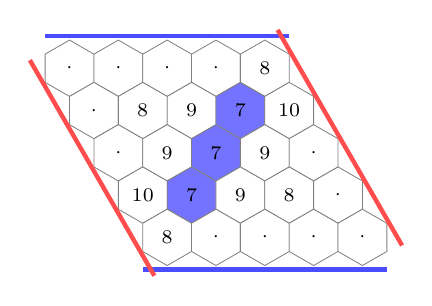
\begin{tikzpicture}[scale=0.62]
\filldraw[fill=white,draw=black!50,line width=0.3pt] (0.000,0.577) -- (-0.500,0.289) -- (-0.500,-0.289) -- (-0.000,-0.577) -- (0.500,-0.289) -- (0.500,0.289) -- cycle;
\node[font=\scriptsize] at (0.000,0.000) {$\cdot$};
\filldraw[fill=white,draw=black!50,line width=0.3pt] (1.000,0.577) -- (0.500,0.289) -- (0.500,-0.289) -- (1.000,-0.577) -- (1.500,-0.289) -- (1.500,0.289) -- cycle;
\node[font=\scriptsize] at (1.000,0.000) {$\cdot$};
\filldraw[fill=white,draw=black!50,line width=0.3pt] (2.000,0.577) -- (1.500,0.289) -- (1.500,-0.289) -- (2.000,-0.577) -- (2.500,-0.289) -- (2.500,0.289) -- cycle;
\node[font=\scriptsize] at (2.000,0.000) {$\cdot$};
\filldraw[fill=white,draw=black!50,line width=0.3pt] (3.000,0.577) -- (2.500,0.289) -- (2.500,-0.289) -- (3.000,-0.577) -- (3.500,-0.289) -- (3.500,0.289) -- cycle;
\node[font=\scriptsize] at (3.000,0.000) {$\cdot$};
\filldraw[fill=white,draw=black!50,line width=0.3pt] (4.000,0.577) -- (3.500,0.289) -- (3.500,-0.289) -- (4.000,-0.577) -- (4.500,-0.289) -- (4.500,0.289) -- cycle;
\node[font=\scriptsize] at (4.000,0.000) {8};
\filldraw[fill=white,draw=black!50,line width=0.3pt] (0.500,-0.289) -- (-0.000,-0.577) -- (0.000,-1.155) -- (0.500,-1.443) -- (1.000,-1.155) -- (1.000,-0.577) -- cycle;
\node[font=\scriptsize] at (0.500,-0.866) {$\cdot$};
\filldraw[fill=white,draw=black!50,line width=0.3pt] (1.500,-0.289) -- (1.000,-0.577) -- (1.000,-1.155) -- (1.500,-1.443) -- (2.000,-1.155) -- (2.000,-0.577) -- cycle;
\node[font=\scriptsize] at (1.500,-0.866) {8};
\filldraw[fill=white,draw=black!50,line width=0.3pt] (2.500,-0.289) -- (2.000,-0.577) -- (2.000,-1.155) -- (2.500,-1.443) -- (3.000,-1.155) -- (3.000,-0.577) -- cycle;
\node[font=\scriptsize] at (2.500,-0.866) {9};
\filldraw[fill=blue!55,draw=black!50,line width=0.3pt] (3.500,-0.289) -- (3.000,-0.577) -- (3.000,-1.155) -- (3.500,-1.443) -- (4.000,-1.155) -- (4.000,-0.577) -- cycle;
\node[font=\scriptsize] at (3.500,-0.866) {7};
\filldraw[fill=white,draw=black!50,line width=0.3pt] (4.500,-0.289) -- (4.000,-0.577) -- (4.000,-1.155) -- (4.500,-1.443) -- (5.000,-1.155) -- (5.000,-0.577) -- cycle;
\node[font=\scriptsize] at (4.500,-0.866) {10};
\filldraw[fill=white,draw=black!50,line width=0.3pt] (1.000,-1.155) -- (0.500,-1.443) -- (0.500,-2.021) -- (1.000,-2.309) -- (1.500,-2.021) -- (1.500,-1.443) -- cycle;
\node[font=\scriptsize] at (1.000,-1.732) {$\cdot$};
\filldraw[fill=white,draw=black!50,line width=0.3pt] (2.000,-1.155) -- (1.500,-1.443) -- (1.500,-2.021) -- (2.000,-2.309) -- (2.500,-2.021) -- (2.500,-1.443) -- cycle;
\node[font=\scriptsize] at (2.000,-1.732) {9};
\filldraw[fill=blue!55,draw=black!50,line width=0.3pt] (3.000,-1.155) -- (2.500,-1.443) -- (2.500,-2.021) -- (3.000,-2.309) -- (3.500,-2.021) -- (3.500,-1.443) -- cycle;
\node[font=\scriptsize] at (3.000,-1.732) {7};
\filldraw[fill=white,draw=black!50,line width=0.3pt] (4.000,-1.155) -- (3.500,-1.443) -- (3.500,-2.021) -- (4.000,-2.309) -- (4.500,-2.021) -- (4.500,-1.443) -- cycle;
\node[font=\scriptsize] at (4.000,-1.732) {9};
\filldraw[fill=white,draw=black!50,line width=0.3pt] (5.000,-1.155) -- (4.500,-1.443) -- (4.500,-2.021) -- (5.000,-2.309) -- (5.500,-2.021) -- (5.500,-1.443) -- cycle;
\node[font=\scriptsize] at (5.000,-1.732) {$\cdot$};
\filldraw[fill=white,draw=black!50,line width=0.3pt] (1.500,-2.021) -- (1.000,-2.309) -- (1.000,-2.887) -- (1.500,-3.175) -- (2.000,-2.887) -- (2.000,-2.309) -- cycle;
\node[font=\scriptsize] at (1.500,-2.598) {10};
\filldraw[fill=blue!55,draw=black!50,line width=0.3pt] (2.500,-2.021) -- (2.000,-2.309) -- (2.000,-2.887) -- (2.500,-3.175) -- (3.000,-2.887) -- (3.000,-2.309) -- cycle;
\node[font=\scriptsize] at (2.500,-2.598) {7};
\filldraw[fill=white,draw=black!50,line width=0.3pt] (3.500,-2.021) -- (3.000,-2.309) -- (3.000,-2.887) -- (3.500,-3.175) -- (4.000,-2.887) -- (4.000,-2.309) -- cycle;
\node[font=\scriptsize] at (3.500,-2.598) {9};
\filldraw[fill=white,draw=black!50,line width=0.3pt] (4.500,-2.021) -- (4.000,-2.309) -- (4.000,-2.887) -- (4.500,-3.175) -- (5.000,-2.887) -- (5.000,-2.309) -- cycle;
\node[font=\scriptsize] at (4.500,-2.598) {8};
\filldraw[fill=white,draw=black!50,line width=0.3pt] (5.500,-2.021) -- (5.000,-2.309) -- (5.000,-2.887) -- (5.500,-3.175) -- (6.000,-2.887) -- (6.000,-2.309) -- cycle;
\node[font=\scriptsize] at (5.500,-2.598) {$\cdot$};
\filldraw[fill=white,draw=black!50,line width=0.3pt] (2.000,-2.887) -- (1.500,-3.175) -- (1.500,-3.753) -- (2.000,-4.041) -- (2.500,-3.753) -- (2.500,-3.175) -- cycle;
\node[font=\scriptsize] at (2.000,-3.464) {8};
\filldraw[fill=white,draw=black!50,line width=0.3pt] (3.000,-2.887) -- (2.500,-3.175) -- (2.500,-3.753) -- (3.000,-4.041) -- (3.500,-3.753) -- (3.500,-3.175) -- cycle;
\node[font=\scriptsize] at (3.000,-3.464) {$\cdot$};
\filldraw[fill=white,draw=black!50,line width=0.3pt] (4.000,-2.887) -- (3.500,-3.175) -- (3.500,-3.753) -- (4.000,-4.041) -- (4.500,-3.753) -- (4.500,-3.175) -- cycle;
\node[font=\scriptsize] at (4.000,-3.464) {$\cdot$};
\filldraw[fill=white,draw=black!50,line width=0.3pt] (5.000,-2.887) -- (4.500,-3.175) -- (4.500,-3.753) -- (5.000,-4.041) -- (5.500,-3.753) -- (5.500,-3.175) -- cycle;
\node[font=\scriptsize] at (5.000,-3.464) {$\cdot$};
\filldraw[fill=white,draw=black!50,line width=0.3pt] (6.000,-2.887) -- (5.500,-3.175) -- (5.500,-3.753) -- (6.000,-4.041) -- (6.500,-3.753) -- (6.500,-3.175) -- cycle;
\node[font=\scriptsize] at (6.000,-3.464) {$\cdot$};
\draw[blue!70,line width=1.6pt] (-0.500,0.657) -- (4.500,0.657);
\draw[blue!70,line width=1.6pt] (1.500,-4.121) -- (6.500,-4.121);
\draw[red!70,line width=1.6pt] (-0.812,0.166) -- (1.738,-4.250);
\draw[red!70,line width=1.6pt] (4.262,0.786) -- (6.812,-3.630);
\end{tikzpicture}
\qquad
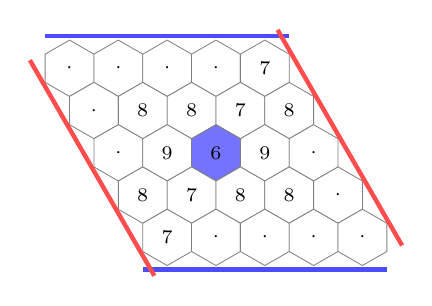
\begin{tikzpicture}[scale=0.62]
\filldraw[fill=white,draw=black!50,line width=0.3pt] (0.000,0.577) -- (-0.500,0.289) -- (-0.500,-0.289) -- (-0.000,-0.577) -- (0.500,-0.289) -- (0.500,0.289) -- cycle;
\node[font=\scriptsize] at (0.000,0.000) {$\cdot$};
\filldraw[fill=white,draw=black!50,line width=0.3pt] (1.000,0.577) -- (0.500,0.289) -- (0.500,-0.289) -- (1.000,-0.577) -- (1.500,-0.289) -- (1.500,0.289) -- cycle;
\node[font=\scriptsize] at (1.000,0.000) {$\cdot$};
\filldraw[fill=white,draw=black!50,line width=0.3pt] (2.000,0.577) -- (1.500,0.289) -- (1.500,-0.289) -- (2.000,-0.577) -- (2.500,-0.289) -- (2.500,0.289) -- cycle;
\node[font=\scriptsize] at (2.000,0.000) {$\cdot$};
\filldraw[fill=white,draw=black!50,line width=0.3pt] (3.000,0.577) -- (2.500,0.289) -- (2.500,-0.289) -- (3.000,-0.577) -- (3.500,-0.289) -- (3.500,0.289) -- cycle;
\node[font=\scriptsize] at (3.000,0.000) {$\cdot$};
\filldraw[fill=white,draw=black!50,line width=0.3pt] (4.000,0.577) -- (3.500,0.289) -- (3.500,-0.289) -- (4.000,-0.577) -- (4.500,-0.289) -- (4.500,0.289) -- cycle;
\node[font=\scriptsize] at (4.000,0.000) {7};
\filldraw[fill=white,draw=black!50,line width=0.3pt] (0.500,-0.289) -- (-0.000,-0.577) -- (0.000,-1.155) -- (0.500,-1.443) -- (1.000,-1.155) -- (1.000,-0.577) -- cycle;
\node[font=\scriptsize] at (0.500,-0.866) {$\cdot$};
\filldraw[fill=white,draw=black!50,line width=0.3pt] (1.500,-0.289) -- (1.000,-0.577) -- (1.000,-1.155) -- (1.500,-1.443) -- (2.000,-1.155) -- (2.000,-0.577) -- cycle;
\node[font=\scriptsize] at (1.500,-0.866) {8};
\filldraw[fill=white,draw=black!50,line width=0.3pt] (2.500,-0.289) -- (2.000,-0.577) -- (2.000,-1.155) -- (2.500,-1.443) -- (3.000,-1.155) -- (3.000,-0.577) -- cycle;
\node[font=\scriptsize] at (2.500,-0.866) {8};
\filldraw[fill=white,draw=black!50,line width=0.3pt] (3.500,-0.289) -- (3.000,-0.577) -- (3.000,-1.155) -- (3.500,-1.443) -- (4.000,-1.155) -- (4.000,-0.577) -- cycle;
\node[font=\scriptsize] at (3.500,-0.866) {7};
\filldraw[fill=white,draw=black!50,line width=0.3pt] (4.500,-0.289) -- (4.000,-0.577) -- (4.000,-1.155) -- (4.500,-1.443) -- (5.000,-1.155) -- (5.000,-0.577) -- cycle;
\node[font=\scriptsize] at (4.500,-0.866) {8};
\filldraw[fill=white,draw=black!50,line width=0.3pt] (1.000,-1.155) -- (0.500,-1.443) -- (0.500,-2.021) -- (1.000,-2.309) -- (1.500,-2.021) -- (1.500,-1.443) -- cycle;
\node[font=\scriptsize] at (1.000,-1.732) {$\cdot$};
\filldraw[fill=white,draw=black!50,line width=0.3pt] (2.000,-1.155) -- (1.500,-1.443) -- (1.500,-2.021) -- (2.000,-2.309) -- (2.500,-2.021) -- (2.500,-1.443) -- cycle;
\node[font=\scriptsize] at (2.000,-1.732) {9};
\filldraw[fill=blue!55,draw=black!50,line width=0.3pt] (3.000,-1.155) -- (2.500,-1.443) -- (2.500,-2.021) -- (3.000,-2.309) -- (3.500,-2.021) -- (3.500,-1.443) -- cycle;
\node[font=\scriptsize] at (3.000,-1.732) {6};
\filldraw[fill=white,draw=black!50,line width=0.3pt] (4.000,-1.155) -- (3.500,-1.443) -- (3.500,-2.021) -- (4.000,-2.309) -- (4.500,-2.021) -- (4.500,-1.443) -- cycle;
\node[font=\scriptsize] at (4.000,-1.732) {9};
\filldraw[fill=white,draw=black!50,line width=0.3pt] (5.000,-1.155) -- (4.500,-1.443) -- (4.500,-2.021) -- (5.000,-2.309) -- (5.500,-2.021) -- (5.500,-1.443) -- cycle;
\node[font=\scriptsize] at (5.000,-1.732) {$\cdot$};
\filldraw[fill=white,draw=black!50,line width=0.3pt] (1.500,-2.021) -- (1.000,-2.309) -- (1.000,-2.887) -- (1.500,-3.175) -- (2.000,-2.887) -- (2.000,-2.309) -- cycle;
\node[font=\scriptsize] at (1.500,-2.598) {8};
\filldraw[fill=white,draw=black!50,line width=0.3pt] (2.500,-2.021) -- (2.000,-2.309) -- (2.000,-2.887) -- (2.500,-3.175) -- (3.000,-2.887) -- (3.000,-2.309) -- cycle;
\node[font=\scriptsize] at (2.500,-2.598) {7};
\filldraw[fill=white,draw=black!50,line width=0.3pt] (3.500,-2.021) -- (3.000,-2.309) -- (3.000,-2.887) -- (3.500,-3.175) -- (4.000,-2.887) -- (4.000,-2.309) -- cycle;
\node[font=\scriptsize] at (3.500,-2.598) {8};
\filldraw[fill=white,draw=black!50,line width=0.3pt] (4.500,-2.021) -- (4.000,-2.309) -- (4.000,-2.887) -- (4.500,-3.175) -- (5.000,-2.887) -- (5.000,-2.309) -- cycle;
\node[font=\scriptsize] at (4.500,-2.598) {8};
\filldraw[fill=white,draw=black!50,line width=0.3pt] (5.500,-2.021) -- (5.000,-2.309) -- (5.000,-2.887) -- (5.500,-3.175) -- (6.000,-2.887) -- (6.000,-2.309) -- cycle;
\node[font=\scriptsize] at (5.500,-2.598) {$\cdot$};
\filldraw[fill=white,draw=black!50,line width=0.3pt] (2.000,-2.887) -- (1.500,-3.175) -- (1.500,-3.753) -- (2.000,-4.041) -- (2.500,-3.753) -- (2.500,-3.175) -- cycle;
\node[font=\scriptsize] at (2.000,-3.464) {7};
\filldraw[fill=white,draw=black!50,line width=0.3pt] (3.000,-2.887) -- (2.500,-3.175) -- (2.500,-3.753) -- (3.000,-4.041) -- (3.500,-3.753) -- (3.500,-3.175) -- cycle;
\node[font=\scriptsize] at (3.000,-3.464) {$\cdot$};
\filldraw[fill=white,draw=black!50,line width=0.3pt] (4.000,-2.887) -- (3.500,-3.175) -- (3.500,-3.753) -- (4.000,-4.041) -- (4.500,-3.753) -- (4.500,-3.175) -- cycle;
\node[font=\scriptsize] at (4.000,-3.464) {$\cdot$};
\filldraw[fill=white,draw=black!50,line width=0.3pt] (5.000,-2.887) -- (4.500,-3.175) -- (4.500,-3.753) -- (5.000,-4.041) -- (5.500,-3.753) -- (5.500,-3.175) -- cycle;
\node[font=\scriptsize] at (5.000,-3.464) {$\cdot$};
\filldraw[fill=white,draw=black!50,line width=0.3pt] (6.000,-2.887) -- (5.500,-3.175) -- (5.500,-3.753) -- (6.000,-4.041) -- (6.500,-3.753) -- (6.500,-3.175) -- cycle;
\node[font=\scriptsize] at (6.000,-3.464) {$\cdot$};
\draw[blue!70,line width=1.6pt] (-0.500,0.657) -- (4.500,0.657);
\draw[blue!70,line width=1.6pt] (1.500,-4.121) -- (6.500,-4.121);
\draw[red!70,line width=1.6pt] (-0.812,0.166) -- (1.738,-4.250);
\draw[red!70,line width=1.6pt] (4.262,0.786) -- (6.812,-3.630);
\end{tikzpicture}

\caption{Value of each opening on the $5\times5$ board: the fewest stones that win ($\delta$, left) and the shortest path that can be forced under Campbell's rules ($\lambda$, right). Blue joins the top and bottom edges. A dot marks an opening that loses ordinary Hex. Shaded cells attain $\delta(5)=7$ and $\lambda(5)=6$.}
\label{fig:tables}
\end{figure}

\begin{figure}[ht]
\centering
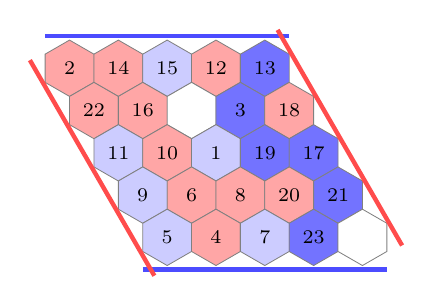
\begin{tikzpicture}[scale=0.62]
\filldraw[fill=red!35,draw=black!50,line width=0.3pt] (0.000,0.577) -- (-0.500,0.289) -- (-0.500,-0.289) -- (-0.000,-0.577) -- (0.500,-0.289) -- (0.500,0.289) -- cycle;
\node[font=\scriptsize] at (0.000,0.000) {2};
\filldraw[fill=red!35,draw=black!50,line width=0.3pt] (1.000,0.577) -- (0.500,0.289) -- (0.500,-0.289) -- (1.000,-0.577) -- (1.500,-0.289) -- (1.500,0.289) -- cycle;
\node[font=\scriptsize] at (1.000,0.000) {14};
\filldraw[fill=blue!20,draw=black!50,line width=0.3pt] (2.000,0.577) -- (1.500,0.289) -- (1.500,-0.289) -- (2.000,-0.577) -- (2.500,-0.289) -- (2.500,0.289) -- cycle;
\node[font=\scriptsize] at (2.000,0.000) {15};
\filldraw[fill=red!35,draw=black!50,line width=0.3pt] (3.000,0.577) -- (2.500,0.289) -- (2.500,-0.289) -- (3.000,-0.577) -- (3.500,-0.289) -- (3.500,0.289) -- cycle;
\node[font=\scriptsize] at (3.000,0.000) {12};
\filldraw[fill=blue!55,draw=black!50,line width=0.3pt] (4.000,0.577) -- (3.500,0.289) -- (3.500,-0.289) -- (4.000,-0.577) -- (4.500,-0.289) -- (4.500,0.289) -- cycle;
\node[font=\scriptsize] at (4.000,0.000) {13};
\filldraw[fill=red!35,draw=black!50,line width=0.3pt] (0.500,-0.289) -- (-0.000,-0.577) -- (0.000,-1.155) -- (0.500,-1.443) -- (1.000,-1.155) -- (1.000,-0.577) -- cycle;
\node[font=\scriptsize] at (0.500,-0.866) {22};
\filldraw[fill=red!35,draw=black!50,line width=0.3pt] (1.500,-0.289) -- (1.000,-0.577) -- (1.000,-1.155) -- (1.500,-1.443) -- (2.000,-1.155) -- (2.000,-0.577) -- cycle;
\node[font=\scriptsize] at (1.500,-0.866) {16};
\filldraw[fill=white,draw=black!50,line width=0.3pt] (2.500,-0.289) -- (2.000,-0.577) -- (2.000,-1.155) -- (2.500,-1.443) -- (3.000,-1.155) -- (3.000,-0.577) -- cycle;
\filldraw[fill=blue!55,draw=black!50,line width=0.3pt] (3.500,-0.289) -- (3.000,-0.577) -- (3.000,-1.155) -- (3.500,-1.443) -- (4.000,-1.155) -- (4.000,-0.577) -- cycle;
\node[font=\scriptsize] at (3.500,-0.866) {3};
\filldraw[fill=red!35,draw=black!50,line width=0.3pt] (4.500,-0.289) -- (4.000,-0.577) -- (4.000,-1.155) -- (4.500,-1.443) -- (5.000,-1.155) -- (5.000,-0.577) -- cycle;
\node[font=\scriptsize] at (4.500,-0.866) {18};
\filldraw[fill=blue!20,draw=black!50,line width=0.3pt] (1.000,-1.155) -- (0.500,-1.443) -- (0.500,-2.021) -- (1.000,-2.309) -- (1.500,-2.021) -- (1.500,-1.443) -- cycle;
\node[font=\scriptsize] at (1.000,-1.732) {11};
\filldraw[fill=red!35,draw=black!50,line width=0.3pt] (2.000,-1.155) -- (1.500,-1.443) -- (1.500,-2.021) -- (2.000,-2.309) -- (2.500,-2.021) -- (2.500,-1.443) -- cycle;
\node[font=\scriptsize] at (2.000,-1.732) {10};
\filldraw[fill=blue!20,draw=black!50,line width=0.3pt] (3.000,-1.155) -- (2.500,-1.443) -- (2.500,-2.021) -- (3.000,-2.309) -- (3.500,-2.021) -- (3.500,-1.443) -- cycle;
\node[font=\scriptsize] at (3.000,-1.732) {1};
\filldraw[fill=blue!55,draw=black!50,line width=0.3pt] (4.000,-1.155) -- (3.500,-1.443) -- (3.500,-2.021) -- (4.000,-2.309) -- (4.500,-2.021) -- (4.500,-1.443) -- cycle;
\node[font=\scriptsize] at (4.000,-1.732) {19};
\filldraw[fill=blue!55,draw=black!50,line width=0.3pt] (5.000,-1.155) -- (4.500,-1.443) -- (4.500,-2.021) -- (5.000,-2.309) -- (5.500,-2.021) -- (5.500,-1.443) -- cycle;
\node[font=\scriptsize] at (5.000,-1.732) {17};
\filldraw[fill=blue!20,draw=black!50,line width=0.3pt] (1.500,-2.021) -- (1.000,-2.309) -- (1.000,-2.887) -- (1.500,-3.175) -- (2.000,-2.887) -- (2.000,-2.309) -- cycle;
\node[font=\scriptsize] at (1.500,-2.598) {9};
\filldraw[fill=red!35,draw=black!50,line width=0.3pt] (2.500,-2.021) -- (2.000,-2.309) -- (2.000,-2.887) -- (2.500,-3.175) -- (3.000,-2.887) -- (3.000,-2.309) -- cycle;
\node[font=\scriptsize] at (2.500,-2.598) {6};
\filldraw[fill=red!35,draw=black!50,line width=0.3pt] (3.500,-2.021) -- (3.000,-2.309) -- (3.000,-2.887) -- (3.500,-3.175) -- (4.000,-2.887) -- (4.000,-2.309) -- cycle;
\node[font=\scriptsize] at (3.500,-2.598) {8};
\filldraw[fill=red!35,draw=black!50,line width=0.3pt] (4.500,-2.021) -- (4.000,-2.309) -- (4.000,-2.887) -- (4.500,-3.175) -- (5.000,-2.887) -- (5.000,-2.309) -- cycle;
\node[font=\scriptsize] at (4.500,-2.598) {20};
\filldraw[fill=blue!55,draw=black!50,line width=0.3pt] (5.500,-2.021) -- (5.000,-2.309) -- (5.000,-2.887) -- (5.500,-3.175) -- (6.000,-2.887) -- (6.000,-2.309) -- cycle;
\node[font=\scriptsize] at (5.500,-2.598) {21};
\filldraw[fill=blue!20,draw=black!50,line width=0.3pt] (2.000,-2.887) -- (1.500,-3.175) -- (1.500,-3.753) -- (2.000,-4.041) -- (2.500,-3.753) -- (2.500,-3.175) -- cycle;
\node[font=\scriptsize] at (2.000,-3.464) {5};
\filldraw[fill=red!35,draw=black!50,line width=0.3pt] (3.000,-2.887) -- (2.500,-3.175) -- (2.500,-3.753) -- (3.000,-4.041) -- (3.500,-3.753) -- (3.500,-3.175) -- cycle;
\node[font=\scriptsize] at (3.000,-3.464) {4};
\filldraw[fill=blue!20,draw=black!50,line width=0.3pt] (4.000,-2.887) -- (3.500,-3.175) -- (3.500,-3.753) -- (4.000,-4.041) -- (4.500,-3.753) -- (4.500,-3.175) -- cycle;
\node[font=\scriptsize] at (4.000,-3.464) {7};
\filldraw[fill=blue!55,draw=black!50,line width=0.3pt] (5.000,-2.887) -- (4.500,-3.175) -- (4.500,-3.753) -- (5.000,-4.041) -- (5.500,-3.753) -- (5.500,-3.175) -- cycle;
\node[font=\scriptsize] at (5.000,-3.464) {23};
\filldraw[fill=white,draw=black!50,line width=0.3pt] (6.000,-2.887) -- (5.500,-3.175) -- (5.500,-3.753) -- (6.000,-4.041) -- (6.500,-3.753) -- (6.500,-3.175) -- cycle;
\draw[blue!70,line width=1.6pt] (-0.500,0.657) -- (4.500,0.657);
\draw[blue!70,line width=1.6pt] (1.500,-4.121) -- (6.500,-4.121);
\draw[red!70,line width=1.6pt] (-0.812,0.166) -- (1.738,-4.250);
\draw[red!70,line width=1.6pt] (4.262,0.786) -- (6.812,-3.630);
\end{tikzpicture}

\caption{A game in which Blue follows the certified centre strategy for $\Hex(5,6)$ and Red plays to make Blue place as many stones as possible. Numbers give the order of moves. Blue uses twelve stones; its connection, completed at move $23$, contains the six-cell path shown dark.}
\label{fig:line5}
\end{figure}

On the $6\times6$ board Red holds $\Hex_9(6)$ against all $36$ openings, and the search finds that only the two central cells of the short diagonal win $\Hex_{10}(6)$ (Figure~\ref{fig:board6}). Red holds $\Hex(6,7)$ against all $36$ openings. Proposition~\ref{prop:lambda6} rests on the search alone: Blue wins $\Hex(6,8)$ after the opening $(3,4)$, a search of $2.9\times10^9$ positions, and Red holds $\Hex(6,8)$ after every opening that is not $(3,4)$ or $(4,3)$. A certificate for this win would be far larger than the others, and we have not replayed one. We have not determined $\lambda^{*}(6)$; we know only $8\le\lambda^{*}(6)\le10$.

\begin{figure}[ht]
\centering
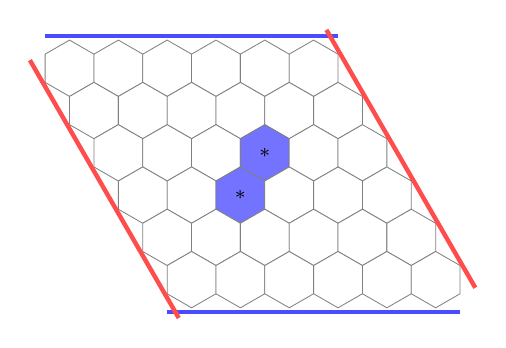
\begin{tikzpicture}[scale=0.62]
\filldraw[fill=white,draw=black!50,line width=0.3pt] (0.000,0.577) -- (-0.500,0.289) -- (-0.500,-0.289) -- (-0.000,-0.577) -- (0.500,-0.289) -- (0.500,0.289) -- cycle;
\filldraw[fill=white,draw=black!50,line width=0.3pt] (1.000,0.577) -- (0.500,0.289) -- (0.500,-0.289) -- (1.000,-0.577) -- (1.500,-0.289) -- (1.500,0.289) -- cycle;
\filldraw[fill=white,draw=black!50,line width=0.3pt] (2.000,0.577) -- (1.500,0.289) -- (1.500,-0.289) -- (2.000,-0.577) -- (2.500,-0.289) -- (2.500,0.289) -- cycle;
\filldraw[fill=white,draw=black!50,line width=0.3pt] (3.000,0.577) -- (2.500,0.289) -- (2.500,-0.289) -- (3.000,-0.577) -- (3.500,-0.289) -- (3.500,0.289) -- cycle;
\filldraw[fill=white,draw=black!50,line width=0.3pt] (4.000,0.577) -- (3.500,0.289) -- (3.500,-0.289) -- (4.000,-0.577) -- (4.500,-0.289) -- (4.500,0.289) -- cycle;
\filldraw[fill=white,draw=black!50,line width=0.3pt] (5.000,0.577) -- (4.500,0.289) -- (4.500,-0.289) -- (5.000,-0.577) -- (5.500,-0.289) -- (5.500,0.289) -- cycle;
\filldraw[fill=white,draw=black!50,line width=0.3pt] (0.500,-0.289) -- (-0.000,-0.577) -- (0.000,-1.155) -- (0.500,-1.443) -- (1.000,-1.155) -- (1.000,-0.577) -- cycle;
\filldraw[fill=white,draw=black!50,line width=0.3pt] (1.500,-0.289) -- (1.000,-0.577) -- (1.000,-1.155) -- (1.500,-1.443) -- (2.000,-1.155) -- (2.000,-0.577) -- cycle;
\filldraw[fill=white,draw=black!50,line width=0.3pt] (2.500,-0.289) -- (2.000,-0.577) -- (2.000,-1.155) -- (2.500,-1.443) -- (3.000,-1.155) -- (3.000,-0.577) -- cycle;
\filldraw[fill=white,draw=black!50,line width=0.3pt] (3.500,-0.289) -- (3.000,-0.577) -- (3.000,-1.155) -- (3.500,-1.443) -- (4.000,-1.155) -- (4.000,-0.577) -- cycle;
\filldraw[fill=white,draw=black!50,line width=0.3pt] (4.500,-0.289) -- (4.000,-0.577) -- (4.000,-1.155) -- (4.500,-1.443) -- (5.000,-1.155) -- (5.000,-0.577) -- cycle;
\filldraw[fill=white,draw=black!50,line width=0.3pt] (5.500,-0.289) -- (5.000,-0.577) -- (5.000,-1.155) -- (5.500,-1.443) -- (6.000,-1.155) -- (6.000,-0.577) -- cycle;
\filldraw[fill=white,draw=black!50,line width=0.3pt] (1.000,-1.155) -- (0.500,-1.443) -- (0.500,-2.021) -- (1.000,-2.309) -- (1.500,-2.021) -- (1.500,-1.443) -- cycle;
\filldraw[fill=white,draw=black!50,line width=0.3pt] (2.000,-1.155) -- (1.500,-1.443) -- (1.500,-2.021) -- (2.000,-2.309) -- (2.500,-2.021) -- (2.500,-1.443) -- cycle;
\filldraw[fill=white,draw=black!50,line width=0.3pt] (3.000,-1.155) -- (2.500,-1.443) -- (2.500,-2.021) -- (3.000,-2.309) -- (3.500,-2.021) -- (3.500,-1.443) -- cycle;
\filldraw[fill=blue!55,draw=black!50,line width=0.3pt] (4.000,-1.155) -- (3.500,-1.443) -- (3.500,-2.021) -- (4.000,-2.309) -- (4.500,-2.021) -- (4.500,-1.443) -- cycle;
\node[font=\scriptsize] at (4.000,-1.732) {$\ast$};
\filldraw[fill=white,draw=black!50,line width=0.3pt] (5.000,-1.155) -- (4.500,-1.443) -- (4.500,-2.021) -- (5.000,-2.309) -- (5.500,-2.021) -- (5.500,-1.443) -- cycle;
\filldraw[fill=white,draw=black!50,line width=0.3pt] (6.000,-1.155) -- (5.500,-1.443) -- (5.500,-2.021) -- (6.000,-2.309) -- (6.500,-2.021) -- (6.500,-1.443) -- cycle;
\filldraw[fill=white,draw=black!50,line width=0.3pt] (1.500,-2.021) -- (1.000,-2.309) -- (1.000,-2.887) -- (1.500,-3.175) -- (2.000,-2.887) -- (2.000,-2.309) -- cycle;
\filldraw[fill=white,draw=black!50,line width=0.3pt] (2.500,-2.021) -- (2.000,-2.309) -- (2.000,-2.887) -- (2.500,-3.175) -- (3.000,-2.887) -- (3.000,-2.309) -- cycle;
\filldraw[fill=blue!55,draw=black!50,line width=0.3pt] (3.500,-2.021) -- (3.000,-2.309) -- (3.000,-2.887) -- (3.500,-3.175) -- (4.000,-2.887) -- (4.000,-2.309) -- cycle;
\node[font=\scriptsize] at (3.500,-2.598) {$\ast$};
\filldraw[fill=white,draw=black!50,line width=0.3pt] (4.500,-2.021) -- (4.000,-2.309) -- (4.000,-2.887) -- (4.500,-3.175) -- (5.000,-2.887) -- (5.000,-2.309) -- cycle;
\filldraw[fill=white,draw=black!50,line width=0.3pt] (5.500,-2.021) -- (5.000,-2.309) -- (5.000,-2.887) -- (5.500,-3.175) -- (6.000,-2.887) -- (6.000,-2.309) -- cycle;
\filldraw[fill=white,draw=black!50,line width=0.3pt] (6.500,-2.021) -- (6.000,-2.309) -- (6.000,-2.887) -- (6.500,-3.175) -- (7.000,-2.887) -- (7.000,-2.309) -- cycle;
\filldraw[fill=white,draw=black!50,line width=0.3pt] (2.000,-2.887) -- (1.500,-3.175) -- (1.500,-3.753) -- (2.000,-4.041) -- (2.500,-3.753) -- (2.500,-3.175) -- cycle;
\filldraw[fill=white,draw=black!50,line width=0.3pt] (3.000,-2.887) -- (2.500,-3.175) -- (2.500,-3.753) -- (3.000,-4.041) -- (3.500,-3.753) -- (3.500,-3.175) -- cycle;
\filldraw[fill=white,draw=black!50,line width=0.3pt] (4.000,-2.887) -- (3.500,-3.175) -- (3.500,-3.753) -- (4.000,-4.041) -- (4.500,-3.753) -- (4.500,-3.175) -- cycle;
\filldraw[fill=white,draw=black!50,line width=0.3pt] (5.000,-2.887) -- (4.500,-3.175) -- (4.500,-3.753) -- (5.000,-4.041) -- (5.500,-3.753) -- (5.500,-3.175) -- cycle;
\filldraw[fill=white,draw=black!50,line width=0.3pt] (6.000,-2.887) -- (5.500,-3.175) -- (5.500,-3.753) -- (6.000,-4.041) -- (6.500,-3.753) -- (6.500,-3.175) -- cycle;
\filldraw[fill=white,draw=black!50,line width=0.3pt] (7.000,-2.887) -- (6.500,-3.175) -- (6.500,-3.753) -- (7.000,-4.041) -- (7.500,-3.753) -- (7.500,-3.175) -- cycle;
\filldraw[fill=white,draw=black!50,line width=0.3pt] (2.500,-3.753) -- (2.000,-4.041) -- (2.000,-4.619) -- (2.500,-4.907) -- (3.000,-4.619) -- (3.000,-4.041) -- cycle;
\filldraw[fill=white,draw=black!50,line width=0.3pt] (3.500,-3.753) -- (3.000,-4.041) -- (3.000,-4.619) -- (3.500,-4.907) -- (4.000,-4.619) -- (4.000,-4.041) -- cycle;
\filldraw[fill=white,draw=black!50,line width=0.3pt] (4.500,-3.753) -- (4.000,-4.041) -- (4.000,-4.619) -- (4.500,-4.907) -- (5.000,-4.619) -- (5.000,-4.041) -- cycle;
\filldraw[fill=white,draw=black!50,line width=0.3pt] (5.500,-3.753) -- (5.000,-4.041) -- (5.000,-4.619) -- (5.500,-4.907) -- (6.000,-4.619) -- (6.000,-4.041) -- cycle;
\filldraw[fill=white,draw=black!50,line width=0.3pt] (6.500,-3.753) -- (6.000,-4.041) -- (6.000,-4.619) -- (6.500,-4.907) -- (7.000,-4.619) -- (7.000,-4.041) -- cycle;
\filldraw[fill=white,draw=black!50,line width=0.3pt] (7.500,-3.753) -- (7.000,-4.041) -- (7.000,-4.619) -- (7.500,-4.907) -- (8.000,-4.619) -- (8.000,-4.041) -- cycle;
\draw[blue!70,line width=1.6pt] (-0.500,0.657) -- (5.500,0.657);
\draw[blue!70,line width=1.6pt] (2.000,-4.987) -- (8.000,-4.987);
\draw[red!70,line width=1.6pt] (-0.812,0.166) -- (2.238,-5.116);
\draw[red!70,line width=1.6pt] (5.262,0.786) -- (8.312,-4.496);
\end{tikzpicture}

\caption{The two openings, marked, that win $6\times6$ Hex with at most ten Blue stones; by our search they are also the only openings that force a path of at most eight cells. They are interchanged by the half-turn.}
\label{fig:board6}
\end{figure}

The sequences now read $\lambda=2,3,5,6,8$ (the last value by Proposition~\ref{prop:lambda6}) and $\delta=2,3,5,7,10$ for $n=2,\dots,6$. Both are strictly increasing, as Campbell's Conjecture~22 predicts.

\section{Remarks}

\paragraph{Where the published argument fails.} The proof of Lemma~5 of~\cite{CPS2026} supposes a centre strategy ``forming a winning path with at most 6 stones'', denotes ``this winning path'' by $\gamma$, and lets Red block it with its second move. This treats $\gamma$ as fixed before Red replies, and it identifies Blue's second and third stones with cells of $\gamma$. An adaptive strategy chooses its path after seeing Red's moves, so this reasoning does not exclude a six-cell win, and the certificate in Table~\ref{tab:cert} exhibits one (Figure~\ref{fig:line5} shows a game). The other parts of that paper are not checked here.

\paragraph{The best opening.} Campbell's Conjecture~18 asserts that the opening in tile $[\lceil n/2\rceil,\lfloor n/2\rfloor]$ achieves $\lambda(n)$~\cite{Campbell2004}. His tile $[b,r]$ is our cell $(r,b)$; in both systems the short diagonal is the set of cells whose coordinates sum to $n+1$, as his example path $\langle[1,4],[2,3],[3,2],[4,1]\rangle$ on the $4\times4$ board shows. Read literally, the conjectured tiles for $n=5$, $[3,2]$ and the alternative $[2,3]$ that Campbell also allows, are our cells $(2,3)$ and $(3,2)$; neither is the centre, and Red holds $\Hex(5,7)$ after both (Figure~\ref{fig:tables}), so the conjecture fails as written for $n=5$. For $n=6$ it is the cell $(3,3)$ on the long diagonal, after which our search finds that Red holds $\Hex(6,8)$. The optimal openings we find are the centre for $n=5$ and the two central cells of the short diagonal for $n=6$, that is, the tile $[\lceil (n+1)/2\rceil,\lfloor (n+1)/2\rfloor]$ and its half-turn image, which may be what was intended.

\paragraph{The two readings.} The rules stated in~\cite{CPS2026}, under which ``a player wins as soon as a connected chain of their own stones joins their two sides'', together with their definition of $\lambda$ through ``every resulting winning path'', amount to the strict game. Under Campbell's rules Theorem~A already fails by the $\Hex(5,6)$ certificate; under the strict reading it fails by the separate $\Hex^{*}(5,6)$ certificate, whose checker keys positions on all Blue stones and stops at the first connection. So the discrepancy with~\cite{CPS2026} does not depend on the rule for long connections. The readings could still differ at larger $n$; our $6\times6$ computation of $\lambda$ uses Campbell's rule.

\paragraph{Open questions.} The next cases are $\lambda^{*}(6)$, $\lambda(7)$ and $\delta(7)$. The KataHex estimate of $25$ moves for $7\times7$ suggests $\delta(7)=13$~\cite{HZY2024}. The value $\delta(5\times\infty)\in\{6,7\}$ left open in~\cite{CPS2026} is not addressed here.

\ifdefined\journalversion
\section*{Research assistance and reproducibility}
Coding agents wrote the search programs, certificate generators and independent checkers, ran the computations, and drafted this manuscript. Valyu DeepResearch supported the literature and priority review. The certificates and checkers in the accompanying repository allow independent replay; the checkers do not use the search code.
\fi

\bibliographystyle{amsplain}
\bibliography{references}
\end{document}
